\documentclass[12pt]{beamer}

\usetheme{Oxygen}
\usepackage{thumbpdf}
\usepackage{wasysym}
% \usepackage{ucs}
\usepackage[utf8]{inputenc}
\usepackage{pgf,pgfarrows,pgfnodes,pgfautomata,pgfheaps,pgfshade}
\usepackage{verbatim}

\pdfinfo
{
  /Title       (Ingeniería de Software)
  /Creator     (TeX)
  /Author      (Sebastián Salazar Molina)
}


\title{Ingeniería de Software}
\subtitle{Introducción}
\author{Sebastián Salazar Molina.}
\institute[INF - UTEM] { Unidad de Informática - Universidad Tecnológica Metropolitana }
\date{27 de Abril de 2015}

\begin{document}

\frame{\titlepage}

\section*{}
\begin{frame}
  \frametitle{Contenidos}
  \tableofcontents[section=1,hidesubsections]
\end{frame}

\AtBeginSection[]
{
  \frame<handout:0>
  {
    \frametitle{Contenidos}
    \tableofcontents[currentsection,hideallsubsections]
  }
}

\AtBeginSubsection[]
{
  \frame<handout:0>
  {
    \frametitle{Contenidos}
    \tableofcontents[sectionstyle=show/hide,subsectionstyle=show/shaded/hide]
  }
}

\newcommand<>{\highlighton}[1]{%
  \alt#2{\structure{#1}}{{#1}}
}

\newcommand{\icon}[1]{\pgfimage[height=1em]{#1}}



%%%%%%%%%%%%%%%%%%%%%%%%%%%%%%%%%%%%%%%%%
%%%%%%%%%% Content starts here %%%%%%%%%%
%%%%%%%%%%%%%%%%%%%%%%%%%%%%%%%%%%%%%%%%%




% Calidad
\section{Gestión de Proyectos}
\subsection{Introducción}

\begin{frame}
 \begin{quote}
Nadie debe empezar un proyecto grande. Empiezas con uno pequeño y trivial y nunca debes esperar que crezca; si lo haces solamente sobre-diseñarás y generalmente pensarás que es más importante de lo que lo es en esta etapa. O peor, puedes asustarte por el tamaño de lo que tu esperas que crezca. Así que empieza pequeño y piensa en los detalles. No pienses acerca de la foto grande y el diseño elegante. Si no resuelve una necesidad inmediata, seguramente está sobre-diseñado. Y no esperes que la gente salte a ayudarte, no es así como estas cosas funcionan. Primero debes tener algo medianamente usable y otros dirán ``hey, esto casi funciona para mí'' y se involucrarán en el proyecto.
 \newline
 \raggedleft{-- Linus Torvald.}
 \end{quote}
\end{frame}


\begin{frame}
 \frametitle{Gestión de Proyectos de Software}
 La gestión de Software, apunta a:
 \begin{itemize}
  \item<2-> Planificar.
  \item<3-> Supervisar.
  \item<4-> Comprobar.
  \item<5-> Ajustarse al presupuesto.
 \end{itemize}
\end{frame}


\begin{frame}
 \frametitle{Piedras en el camino.}
 Existen un conjunto de actividades que dificultan la gestión de proyectos de Software.
 \begin{itemize}
  \item<2-> La intangibilidad del Software.
  \item<3-> La falta de estándares.
  \item<4-> La unicidad de los proyectos.
 \end{itemize}
\end{frame}


\section{Actividades}
\subsection{Introducción}

\begin{frame}
 \frametitle{Actividades}
 Existen un conjunto de actividades ampliamente aceptadas para la gestión del proyectos.
 \begin{itemize}
  \item<2-> Propuesta (inicio).
  \item<3-> Planificación del proyecto.
  \item<4-> Estimación de costos del proyecto.
  \item<5-> Control y Retroalimentación del proyecto.
  \item<6-> Selección del personal.
  \item<7-> Cierre.
 \end{itemize}
\end{frame}


\subsection{Propuesta}
\begin{frame}
 \frametitle{Propuesta}
 La propuesta es el documento, donde se describen los objetivos del proyecto y la forma en que se trabajaran. También se pueden expresar costos y estimaciones apriori.
 \newline
 La redacción de las propuestas es una tarea muy delicada.
\end{frame}


\subsection{Planificación.}

\begin{frame}
 \frametitle{Planificación del proyecto.}
 La clave de un proyecto es anticiparse a los problemas, logrando transformar amenazas en oportunidades.
 \newline
 La herramientas son los \alert{planes}. Se debe evaluar con sumo cuidado tanto nuestras capacidades cómo las circunstancias, el objetivo es poder trazar un plan de trabajo coherente con la realidad, a la vez, que nos permite tener planes de contingencia ante problemas esperados.
\end{frame}


\begin{frame}
 \frametitle{Plan de Trabajo}
 El plan de trabajo se debe componer de una serie de tareas que deben ser bien \alert{comprendidas}, por el equipo de trabajo.
 \begin{itemize}
  \item<2-> Definición de Objetivos y Alcances, Introducción.
  \item<3-> Levantar Requerimientos.
  \item<4-> Planificar el trabajo. Definir los \alert{hitos} y las entregas.
  \item<5-> Analizar riesgos potenciales.
  \item<6-> Controlar y verificar los distintos procesos.
 \end{itemize}
\end{frame}


\begin{frame}
 \frametitle{Objetivos y Alcances}
 Se define de que se trata el proyecto y a qué nos \alert{comprometemos}.
\end{frame}


\begin{frame}
 \frametitle{Levantar Requerimientos}
 Determinamos las necesidades que se deben cubrir con la solución a desarrollar.
\end{frame}


\begin{frame}
 \frametitle{Planificar}
 Es la etapa más compleja y la que requiere más experiencia, consiste en aprovechar al máximo los recursos que se disponen para el proyecto (El personal, los recursos y el tiempo).
\end{frame}


\begin{frame}
 \frametitle{Análisis de Riesgos.}
 Un riesgo es cualquier actividad o circunstancia que pudiera afectar el éxito del proyecto.
 \newline
 Existen básicamente 3 tipos de Riesgos:
 
 \begin{itemize}
  \item<2-> Riesgos del proyecto.
  \item<3-> Riesgos del Software.
  \item<4-> Riesgos del Negocio.
 \end{itemize}
 
\end{frame}


\begin{frame}
 \frametitle{Gestión de Riesgos.}
 Comprende las siguientes actividades:
 
 \begin{itemize}
  \item<2-> Identificación.
  \item<3-> Análisis.
  \item<4-> Confección de planes de contingencia.
  \item<5-> Control y Seguimiento de Riesgos.
 \end{itemize}
 
\end{frame}


\subsection{Control y Seguimiento}

\begin{frame}
 \frametitle{Control y Seguimiento del proyecto.}
 Son todas aquellas actividades que me indican la ``salud'' del proyecto.
\end{frame}


\subsection{Cierre}

\begin{frame}
 \frametitle{Cierre}
 Las actividades de Cierre buscan documentar la experiencia adquirida con el proyecto.
\end{frame}


\begin{frame}
 \begin{quote}
Hay un peligro complementario en prever el futuro y tratar de predecirlo. A menudo quedamos convencidos de que las sorpresas del ayer determinarán lo que pasará mañana. [...] Pero para bien o para mal, el mañana es una novedad. Es la novedad de la casualidad, cosas que se reúnen de una manera que no podemos predecir. [...] Lo que hace el mañana es el hecho de que no puede ser predicho hoy; no tiene relación con lo actual
 \newline
 \raggedleft{-- Robert Oppenheimer.}
 \end{quote}
\end{frame}



\section{PMBOK}
\subsection{Introducción}


\begin{frame}
\frametitle{Introducción}
El PMBOK es el estándar más ampliamente reconocido para manejar y administrar proyectos, es una obra con un agudo sentido práctico. En donde se definen un conjunto de buenas prácticas y se sugieren metodologías de trabajo que han probado ser exitosas, aunque se hace un gran hincapié en que todos los proyectos son diferentes y que no existe una única receta mágica para su desarrollo.  
\end{frame}

\subsection{Definiciones}
\begin{frame}
 \frametitle{Definición de Proyecto}
El PMBOK define un proyecto como \alert{``un esfuerzo temporal de recursos limitados para crear un producto o servicio único. El
carácter temporal significa que los proyectos tienen un inicio y término determinados''}.
\end{frame}


\begin{frame}
 \frametitle{Etapas de un proyecto}
El PMBOK define 5 etapas características de un proyecto:
\begin{center}
 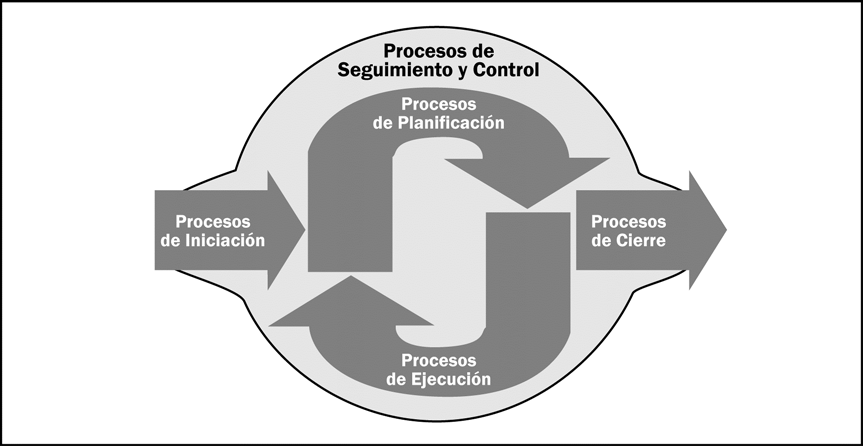
\includegraphics[scale=0.35]{img/pmbok.png}
\end{center}
\end{frame}


\begin{frame}
\frametitle{Dimensiones del proyecto.}
Principales perspectivas:
\begin{itemize}
 \item<2-> Personas involucradas.
 \item<3-> Datos.
 \item<4-> Metodologías y Técnicas de trabajo.
 \item<5-> Recursos
\end{itemize}
\end{frame}




\section{Procesos}
\subsection{Iniciación}


\begin{frame}
 \begin{quote}
  Hay muchas cosas en la vida más importantes que el dinero. ¡Pero cuestan tanto!.
 \newline
 \newline
 \raggedleft{-- Groucho Marx.}
 \end{quote}
\end{frame}




\begin{frame}
 \frametitle{Iniciación}
 Se deben estudiar los siguientes elementos:
 \begin{itemize}
  \item<2-> Autorización (Buscar Sponsor, detectar interesados, involucrados y gente comprometida).
  \item<3-> Establecer los recursos iniciales con que cuenta el proyecto.
  \item<4-> Definir el equipo de trabajo.
 \end{itemize}
\end{frame}


\subsection{Planificación}

\begin{frame}
 \begin{quote}
 Para tener éxito, la planificación sola es insuficiente. Uno debe improvisar también.
 \newline
 \newline
 \raggedleft{-- Isaac Asimov.}
 \end{quote}
\end{frame}


\begin{frame}
 \frametitle{Planificación}
La idea principal de la planificación, es anticiparse a los problemas eventuales que puedan surgir para
implantación del proyecto, la realización de planes de acción, se enmarca en la
definición de tareas y actividades claras que pueden ser seguidas con facilidad por
parte del equipo de trabajo.
\end{frame}


\begin{frame}
 \frametitle{Actividades}
 \begin{itemize}
  \item<1-> Desarrollar los planes de acción.
  \item<2-> Recopilar Requisitos y Requerimientos.
  \item<3-> Definir Alcances.
  \item<4-> Desglosar el trabajo.
  \item<5-> Definir y Secuenciar las Actividades.
 \end{itemize}
\end{frame}


\begin{frame}
 \frametitle{Actividades}
 \begin{itemize}
  \item<1-> Estimar los recursos por actividad, junto con el tiempo necesario (hacer cronograma).
  \item<2-> Definir el presupuesto.
  \item<3-> Planificar la Calidad.
  \item<4-> Planificar Riesgos.
  \item<5-> Planificar Adquisiciones.
 \end{itemize}
\end{frame}


\subsection{Ejecución}


\begin{frame}
 \begin{quote}
 Algo malo debe tener el trabajo porque si no, los ricos lo habrían acaparado.
 \newline
 \newline
 \raggedleft{-- Mario Moreno - Cantinflas.}
 \end{quote}
\end{frame}


\begin{frame}
 \frametitle{Ejecución}
 La mayor parte de un proyecto se lleva a cabo en esta etapa, usualmente consume un
80\% del tiempo estimado, el objetivo es realizar el trabajo definido en la
planificación, a fin de cumplir con las especificaciones del producto de Software.
\end{frame}


\begin{frame}
 \frametitle{Actividades}
 \begin{itemize}
  \item<2-> Gestionar la Ejecución del proyecto.
  \item<3-> Gestionar el Aseguramiento de la calidad (proceso de mejora continua).
  \item<4-> Adquirir Equipamiento (si fuese necesario).
  \item<5-> Gestionar expectativas.
 \end{itemize}
\end{frame}





\subsection{Seguimiento y Control}

\begin{frame}
 \begin{quote}
 No podemos resolver problemas pensando de la misma manera que cuando los creamos..
 \newline
 \newline
 \raggedleft{-- Albert Einstein.}
 \end{quote}
\end{frame}

\begin{frame}
 \frametitle{Seguimiento y Control.}
 En la etapa de seguimiento y control, se definen los procesos para dar seguimiento,
analizar y regular el progreso y el desempeño del proyecto.
\end{frame}


\begin{frame}
 \frametitle{Seguimiento y Control.}
  Nuestros objetivos son avanzar en el cumplimiento de las tareas e identificar los problemas que pueden
surgir mientras desarrollamos el proyecto, para poder aplicar las medidas correctivas.
\end{frame}


\begin{frame}
 \frametitle{Actividades}
 \begin{itemize}
  \item<2-> Controlar Cambios (evolución del Software).
  \item<3-> Comprobar nuestra correlación con el alcance.
  \item<4-> Controlar los tiempos.
  \item<5-> Controlar el presupuesto.
 \end{itemize}
\end{frame}


\begin{frame}
 \frametitle{Actividades}
 \begin{itemize}
  \item<1-> Controlar la calidad.
  \item<2-> Controlar los riesgos.
  \item<3-> Administrar Adquisiciones.
 \end{itemize}

\end{frame}


\subsection{Cierre}

\begin{frame}
 \begin{quote}
 La vida es el arte de sacar conclusiones suficientes a partir de datos insuficientes.
 \newline
 \newline
 \raggedleft{-- Samuel Butler.}
 \end{quote}
\end{frame}

\begin{frame}
 \frametitle{Conclusiones}
 Establecer y documentar la experiencia que nos dejó el proyecto (particularmente los obstáculos y elementos negativos). Valorar los puntos positivos, obtener la aprobación del cliente.
 \pause
 \newline
 Opcionalmente, actualizar practicas y procesos. Definir Trabajo Futuro (TODO).
\end{frame}


\section{Áreas de Conocimiento}
\subsection{Introducción}

\begin{frame}
 \frametitle{Áreas de Conocimiento.}
 
 Las áreas del conocimiento, son el conjunto de buenas prácticas que nos permitirán llegar a puerto en nuestros proyectos.
 \pause
 En la Quinta Edición de la Guía PMBOK (2012), se definen 10 áreas de conocimiento. Cada una de las diez áreas de conocimiento contiene los procesos (un total de 47) que deben llevarse a cabo dentro de su disciplina con el fin de lograr un programa de gestión de proyectos eficaz. Cada uno de estos procesos también cae en uno de los cinco grupos de procesos básicos.
\end{frame}


\begin{frame}
 \frametitle{Áreas de Conocimiento}
 \begin{itemize}
  \item<2-> 1. Gestión de la Integración del Proyecto.
  \item<2-> 2. Gestión del Alcance del Proyecto.
  \item<3-> 3. Gestión del Tiempo del Proyecto.
  \item<4-> 4. Gestión de los Costos del Proyecto.
  \item<5-> 5. Gestión de la Calidad del Proyecto.
 \end{itemize}
\end{frame}


\begin{frame}
 \frametitle{Áreas de Conocimiento}
 \begin{itemize}  
  \item<1-> 6. Gestión de los Recursos Humanos del Proyecto.
  \item<2-> 7. Gestión de las Comunicaciones del Proyecto.
  \item<3-> 8. Gestión de los Riesgos del Proyecto.
  \item<4-> 9. Gestión de las Adquisiciones del Proyecto.
  \item<5-> 10. Gestión de los Interesados.
 \end{itemize}
\end{frame}

\subsection{Áreas de Conocimiento.}


\begin{frame}
 \frametitle{Gestión de la Integración del Proyecto.}
 En esta área se agrupan los conocimientos necesarios para que todos los elementos del proyecto estén coordinados adecuadamente.
 \begin{itemize}
  \item<2-> Desarrollar el Acta de Constitución del Proyecto (Proceso de Inicio)
  \item<3-> Desarrollar el Plan para la Dirección del Proyecto (Proceso de Planificación)
  \item<4-> Dirigir y Gestionar la ejecución del Proyecto (Proceso de Ejecución)
  \item<5-> Monitorizar y Controlar el trabajo del Proyecto (Proceso de Seguimiento y Control)
  \item<6-> Realizar el Control Integrado de Cambios (Proceso de Seguimiento y Control)
  \item<7-> Cerrar Proyecto o Fase (Proceso de Cierre)
 \end{itemize}
\end{frame}



\begin{frame}
 \frametitle{Gestión del Alcance del Proyecto.}
 En esta área se agrupan los conocimientos necesarios para garantizar, que se realiza todo el trabajo necesario para la ejecución del proyecto, ni más, ni menos.
 \begin{itemize}
  \item<2-> Plan de Gestión del Alcance (Proceso de Planificación)
  \item<2-> Recopilar requisitos (Proceso de Planificación)
  \item<3-> Definir el Alcances (Proceso de Planificación)
  \item<4-> Crear la Estructura del Desglose de Trabajo (EDT) (Proceso de Planificación)
  \item<5-> Verificar el Alcances (Proceso de Seguimiento y Control)
  \item<6-> Controlar el Alcance (Proceso de Seguimiento y Control)
 \end{itemize}
\end{frame}



\begin{frame}
 \frametitle{Gestión del Tiempo del Proyecto.}
 En esta área se agrupan los conocimientos necesarios para garantizar, que se realiza el proyecto se terminará en los plazos establecidos.
 \begin{itemize}
  \item<2-> Plan de Gestión del Cronograma (Proceso de Planificación)
  \item<3-> Definir las actividades (Proceso de Planificación)
  \item<4-> Secuenciar las actividades (Proceso de Planificación)
  \item<5-> Estimar los Recursos de las Actividades (Proceso de Planificación)
  \item<6-> Estimar la Duración de las Actividades (Proceso de Planificación)
  \item<7-> Desarrollar el Cronograma (Proceso de Planificación)
  \item<8-> Controlar el Cronograma (Proceso de Seguimiento y Control)
 \end{itemize}
\end{frame}



\begin{frame}
 \frametitle{Gestión de los Costos del Proyecto.}
 En esta área se agrupan los conocimientos necesarios para garantizar, que el proyecto se ajusta al presupuesto estimado.
 \begin{itemize}
  \item<2-> Plan de Gestión de Costos (Proceso de Planificación)
  \item<3-> Estimar los Costos (Proceso de Planificación)
  \item<4-> Determinar el Presupuesto (Proceso de Planificación)
  \item<5-> Controlar los Costos (Proceso de Seguimiento y Control)
 \end{itemize}
\end{frame}



\begin{frame}
 \frametitle{Gestión de la Calidad del Proyecto.}
 En esta área se agrupan los conocimientos necesarios para garantizar, que el proyecto va a satisfacer las necesidades para lo cual fue desarrollado.
 \begin{itemize}
  \item<2-> Plan de Gestión de la Calidad (Proceso de Planificación)
  \item<3-> Realizar el Aseguramiento de Calidad (Proceso de Ejecución)
  \item<4-> Realizar el Control de Calidad (Proceso de Seguimiento y Control)
 \end{itemize}
\end{frame}



\begin{frame}
 \frametitle{Gestión de los Recursos Humanos del Proyecto.}
 En esta área se agrupan los conocimientos necesarios para hacer uso eficiente del equipo humano del proyecto.
 \begin{itemize}
  \item<2-> Plan de Gestión de Recursos Humanos (Proceso de Planificación)
  \item<3-> Adquirir el Equipo del Proyecto (Proceso de Ejecución) 
  \item<4-> Desarrollar el Equipo del Proyecto (Proceso de Ejecución)
  \item<5-> Dirigir el Equipo del Proyecto (Proceso de Ejecución)
 \end{itemize}
\end{frame}



\begin{frame}
 \frametitle{Gestión de las Comunicaciones del Proyecto.}
 En esta área se agrupan los conocimientos necesarios para garantizar la generación, colección, diseminación, almacenamiento y la disposición final de la información del proyecto de una forma adecuada y en los plazos estipulados.
 \begin{itemize}
  \item<2-> Plan de Gestión de la Comunicación (Proceso de Planificación)
  \item<3-> Gestionar la Comunicación (Proceso de Ejecución)
  \item<4-> Controlar la Comunicación (Proceso de Seguimiento y Control)
 \end{itemize}
\end{frame}


\begin{frame}
 \frametitle{Gestión de los Riesgos del Proyecto.}
 En esta área se agrupan los conocimientos necesarios para la identificación, análisis, y respuesta a los riesgos del proyecto.
 \begin{itemize}
  \item<2-> Plan de Gestión de Riesgos (Proceso de Planificación)
  \item<3-> Identificar los Riesgos (Proceso de Planificación)
  \item<4-> Realizar el Análisis \href{http://lema.rae.es/drae/srv/search?key=cualitativo}{Cualitativo} de Riesgos (Proceso de Planificación)
  \item<5-> Realizar el Análisis \href{http://lema.rae.es/drae/srv/search?key=cuantitativo}{Cuantitativo} de Riesgos (Proceso de Planificación)
  \item<6-> Planificar la Respuesta a los riesgos (Proceso de Planificación)
  \item<7-> Monitorizar y Controlar los Riesgos (Proceso de Seguimiento y Control)
 \end{itemize}
\end{frame}


\begin{frame}
 \frametitle{Gestión de las Adquisiciones del Proyecto.}
 En esta área se agrupan los conocimientos necesarios para la adquisición de bienes y servicios de fuera del equipo del proyecto.
 \begin{itemize}
  \item Plan de Gestión de las Adquisiciones (Proceso de Planificación)
  \item Efectuar las Adquisiciones (Proceso de Ejecución)
  \item Controlar las Adquisiciones (Proceso de Seguimiento y Control)
  \item Cerrar (Finalizar) las Adquisiciones (Proceso de Cierre)
 \end{itemize}
\end{frame}


\begin{frame}
 \frametitle{Gestión de los Interesados.}
 En esta área se agrupan los conocimientos necesarios para interactuar y obtener el mejor resultado de los involucrados en el proyecto.
 \begin{itemize}
  \item<2-> Identificar Involucrados (Stakeholders) (Proceso de Inicio)
  \item<3-> Plan de Gestión de Involucrados (Proceso de Planificación)
  \item<4-> Administrar a los Involucrados (Proceso de Ejecución)
  \item<5-> Controlar a los Involucrados (Proceso de Seguimiento y Control)
 \end{itemize}
\end{frame}



\subsection{Resumen}

\begin{frame}
  \frametitle{Resumen}
  \begin{center}
    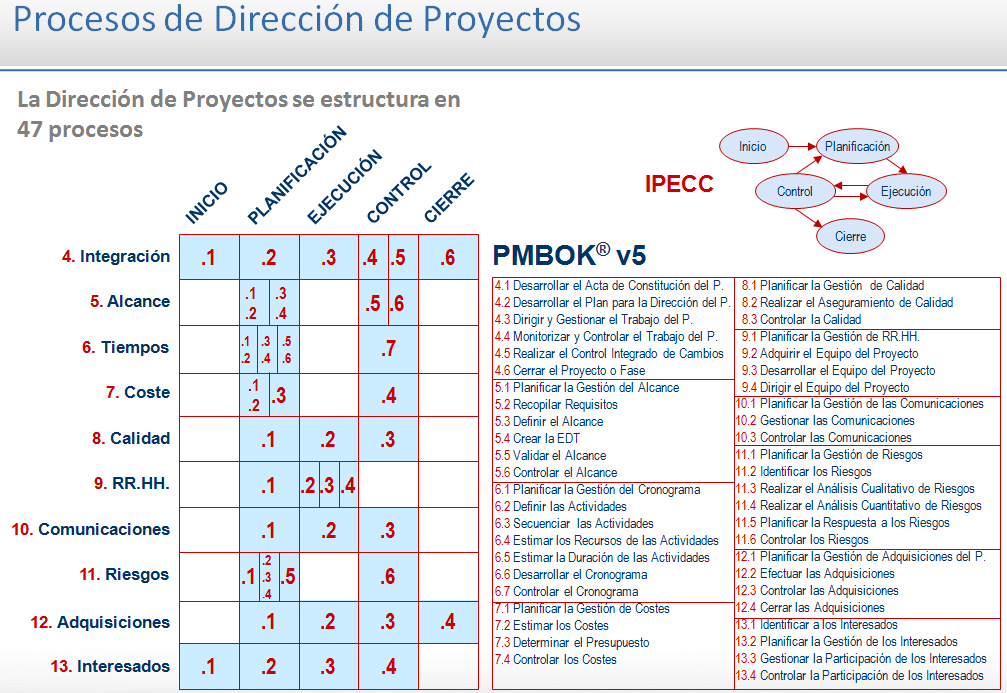
\includegraphics[scale=0.35]{img/conocimiento.png}
  \end{center}
\end{frame}



\frame{
  \vspace{2cm}
  {\huge ¿ Preguntas ?}

  \vspace{3cm}
  \begin{flushright}
    Sebastián Salazar Molina

    \structure{\footnotesize{sebasalazar@gmail.com}}
  \end{flushright}
}

\end{document}
